\documentclass[a4paper]{article}
\usepackage{url}
\usepackage{multirow}
\usepackage{INTERSPEECH2021}
\usepackage{cite}
\usepackage{tablefootnote}
\usepackage{color}
\usepackage{booktabs}
\usepackage{graphicx} 
\usepackage{epstopdf, multirow}
\usepackage{pifont}
\usepackage{footnote}
\usepackage{soul}
\usepackage{amssymb}% http://ctan.org/pkg/amssymb
\usepackage{pifont}%
%http://ctan.org/pkg/pifont
% \usepackage{biblatex}
% \renewcommand*{\bibfont}{\footnotesize}
\newcommand{\cmark}{\ding{51}}%
\newcommand{\xmark}{\ding{55}}%
% \usepackage{comment}
\newcommand{\textoverline}[1]{$\overline{\mbox{#1}}$}
\usepackage{todonotes}
\setlength{\intextsep}{1pt plus 0pt minus 3pt} %distance between floats on the top or the bottom and the text
\setlength{\textfloatsep}{1pt plus 0pt minus 4pt}%distance between two floats
\setlength{\floatsep}{1pt plus 0pt minus 2pt}%distance

\title{Learning Language-independent Subword Discriminative Feature Representation for Unsupervised Acoustic Unit Discovery}
\name{Siyuan Feng, Odette Scharenborg}
%The maximum number of authors in the author list is twenty. If the number of contributing authors is more than twenty, they should be listed in a footnote or in acknowledgement section, as appropriate.
\address{
  Multimedia Computing Group, 
  Delft University of Technology, Delft,  the Netherlands}% \\
 %$^2$Department of Electronic Engineering, The Chinese University of Hong Kong, Hong Kong}
\email{\{s.feng, o.e.scharenborg\}@tudelft.nl}

\begin{document}

\maketitle
% 
\begin{abstract}
% \todo[inline]{Placeholder text, to be written later}
This paper tackles the problem of discovering  phoneme-like acoustic units for a language with only unlabeled speech data available. Unlike   past studies which usually proposed integrated approaches, we propose a two-stage approach: the first stage learns a   subword-discriminative feature  representation and the second stage applies clustering   to the learned representation and obtains phoneme-like  clusters as the discovered acoustic units. In the first stage, a recently proposed unsupervised subword modeling method is leveraged and improved by replacing a monolingual out-of-domain (OOD) ASR system with a multilingual one to create a more language-independent subword-discriminative representation. In the second stage,  segment-level k-means is adopted, and two segment representation methods are compared. Experiments   on a very low-resource Mboshi database show that our approach outperforms state of the art in both NMI and F-score. The advantages of a multilingual ASR over a monolingual one are shown both in providing OOD phone labels and in estimating   phone boundaries, with the former being more prominent. A simple average based method is competitive to a downsampling method in obtaining segment representations.
The 16\% NMI performance gap between our systems with and without knowing golden phone boundaries suggests future research towards improving  phone boundary estimation. Our  approach achieves the best performance when the cluster number is set around 50 and 70.
 \end{abstract}
\noindent\textbf{Index Terms}:  
Acoustic unit discovery, unsupervised subword modeling, zero-resource
\section{Introduction}
Recent advancements of automatic speech recognition (ASR)   \cite{dahl2012context,Li2020comparison} are attributed from two main factors: successful application of deep neural networks (DNNs) and large amounts of  annotated speech data for model training. There are around $7,000$ spoken languages in the world \cite{austin2011cambridge}, most of which   lack transcribed speech resources \cite{speech2020scharenborg}. In addition, linguistic knowledge about such  \textit{low-resource} languages is incomplete or even non-existent. Conventional supervised acoustic modeling strategies \cite{dahl2011context,chan2016listen,graves2014towards,graves2012RNN_T} cannot be applied directly. As a result, current high-performance ASR systems are available only for a very small number of languages \cite{feng2021how}.

To facilitate ASR for low-resource languages,  unsupervised acoustic modeling  has been gaining a growing research interest  recently \cite{lee2012a,I3EWang,chen2015parallel,ondel2017bayesian,Chen2020unsupervised}.  unsupervised acoustic modeling seeks to model basic speech units that represent  all the sounds in a target language by making a  \textit{zero-resource} assumption  \cite{versteegh2015zero}: for the target language, only speech recordings are available while transcriptions and phoneme inventory (and its size) information are unknown. 

There are two mainstream research strands in unsupervised acoustic modeling. The first strand, named as \textit{acoustic unit discovery (AUD)} \cite{ondel2016variational,lee2012a}, formulates the problem as discovering a finite set of phoneme-like acoustic units \cite{lee2012a,I3EWang,Ondel2019Bayesian}. 
% Studies on the AUD task can be traced back to early 2010s \cite{lee2012a,Wang2013unsup_mining}. 
The second strand, referred to as \textit{unsupervised subword modeling (USM)} \cite{versteegh2015zero,dunbar2017zero,Dunbar2019}, formulates the problem as learning a frame-level feature representation  that can distinguish subword units (phonemes)  and is robust to speaker variation \cite{chen2015parallel,oord2017neural,heck2017feature}. 
Studies on the USM task were mostly driven by the  Zero Resource Speech Challenges (ZeroSpeech)  \cite{versteegh2015zero,dunbar2017zero,Dunbar2019,Dunbar2020zero}. 
In essence, the USM task can be considered as learning an intermediate representation towards achieving the goal in AUD \cite{Feng2019combining}. 

This study addresses the AUD task. Past studies  (see Section \ref{sec:related_works})   usually directly focused  on the AUD problem  and proposed integrated approaches  \cite{lee2012a,Ondel2019Bayesian,baevski2020vqwav2vec}. In contrast, the present study proposes a two-stage learning framework: the first stage learns a frame-level subword-discriminative  feature representation  (i.e. the USM task); the second stage  applies clustering techniques to the  learned  representation to obtain a set of clusters as the discovered acoustic units. 
% The advantage of the first stage is that,
Comparing to spectral   representations e.g. MFCC,  in a subword-discriminative feature representation, speech of the same phoneme are closer while speech of different phonemes are further apart \cite{dunbar2017zero}. This is a highly desired property in     clustering based phoneme-like unit discovery \cite{I3EWang,Bhati2019unsupervised}, which motivates us to  propose such a two-stage learning framework.

Specifically, in the first stage of the framework, we leverage and   improve an USM approach  proposed by our previous study \cite{feng2020unsupervised}. This approach trains  an autoregressive predictive coding (APC)  model \cite{Chung2019} followed by a cross-lingual DNN model to  extract the bottleneck feature  (BNF)  as the   subword-discriminative representation. 
By exploiting an out-of-domain (OOD) language's resources, this approach achieved state of the art in USM \cite{feng2020unsupervised,feng2020effectiveness}. 
We further improve this approach by exploiting multiple OOD languages' resources during DNN  training, with the hope of building a more language-independent cross-lingual DNN than \cite{feng2020unsupervised} to benefit target in-domain language acoustic modeling.
% modeling the target unknown language.
Moreover, unlike in \cite{feng2020unsupervised} where the APC was found crucial in the USM task, the present study shows  that APC does not affect the AUD performance. To our knowledge the  approach in \cite{feng2020unsupervised} has not been studied for the AUD task.
% on ZeroSpeech 2017 \cite{dunbar2017zero} as well as Libri-light \cite{kahn2019librilight} databases. 
In the second stage of our system framework,   $k$-means algorithm is adopted in speech segment clustering, where segment boundaries are estimated via OOD ASR systems. 
To represent arbitrary-length segments as fixed-dimension vectors, 
% A key issue in segment clustering is to represent arbitrary-length segments as fixed-dimension vectors \cite{levin2013fixed}. 
we compare  an average-based method \cite{I3EWang} and a downsampling method \cite{levin2013fixed}. 
While the latter method was more recommended by recent works, we do not find its superiority. 
Both methods outperform a frame-level clustering baseline.  
Experiments\footnote{Code resources for this study are under preparation and will be made open-sourced soon.} conducted  on a very low-resource Mboshi corpus  \cite{Godard2018mboshi} ($4.5$ hours of unlabeled speech)   demonstrate that our   system outperforms   state of the art in the AUD task \cite{Yusuf2020hierarchical,Ondel2019Bayesian}.
% , and the advantage of applying a language-independent OOD ASR is mainly on improving the phonetic relevance of the discovered units, rather than on improving phone boundary estimation.
% It is expected that  subword-discriminative feature representations are highly desired for  feature clustering in the AUD task \cite{feng2016exploit}

\section{Related works}
\label{sec:related_works}
There are two main types of approaches to  the AUD task. The first type adopts  self-supervised representation learning algorithms and apply a quantization layer to obtain a finite set of discovered acoustic units \cite{oord2017neural,baevski2020vqwav2vec,Niekerk2020vector}. The second type adopts Bayesian non-parametric versions of the hidden Markov model (HMM) \cite{lee2012a,Ondel2019Bayesian,Yusuf2020hierarchical}. The combination of self-supervised learning and Bayesian approaches was also studied \cite{Ebbers2017,Glarner2018Full,ondel2018bayesian}.




\section{Proposed two-stage approach}
% The two stages of our proposed approach to the AUD task are described 
% Our  proposed approach to the AUD task consists of two stages. The first stage learns a subword-discriminative feature representation. The second stage applies $k$-means algorithm to cluster target speech based on the learned feature representation and obtain a finite set of phoneme-like acoustic units. The two stages are described 
% in Sections \ref{subsec:approach_1st} and \ref{subsec:approach_2nd_stage} respectively.
\subsection{Stage 1: subword-discriminative feature learning}
\label{subsec:approach_1st}
The goal of this stage is to learn a frame-level subword-discriminative feature representation.
% feature representation that can distinguish subword units of a target language and is robust to speaker variation. 
The approach in \cite{feng2020unsupervised} is adopted, modified and improved in this study.
% with modifications and improvements. 
The  general framework of this approach is illustrated in Figure \ref{fig:framework_1st}.
\begin{figure}[!t]
    \centering
    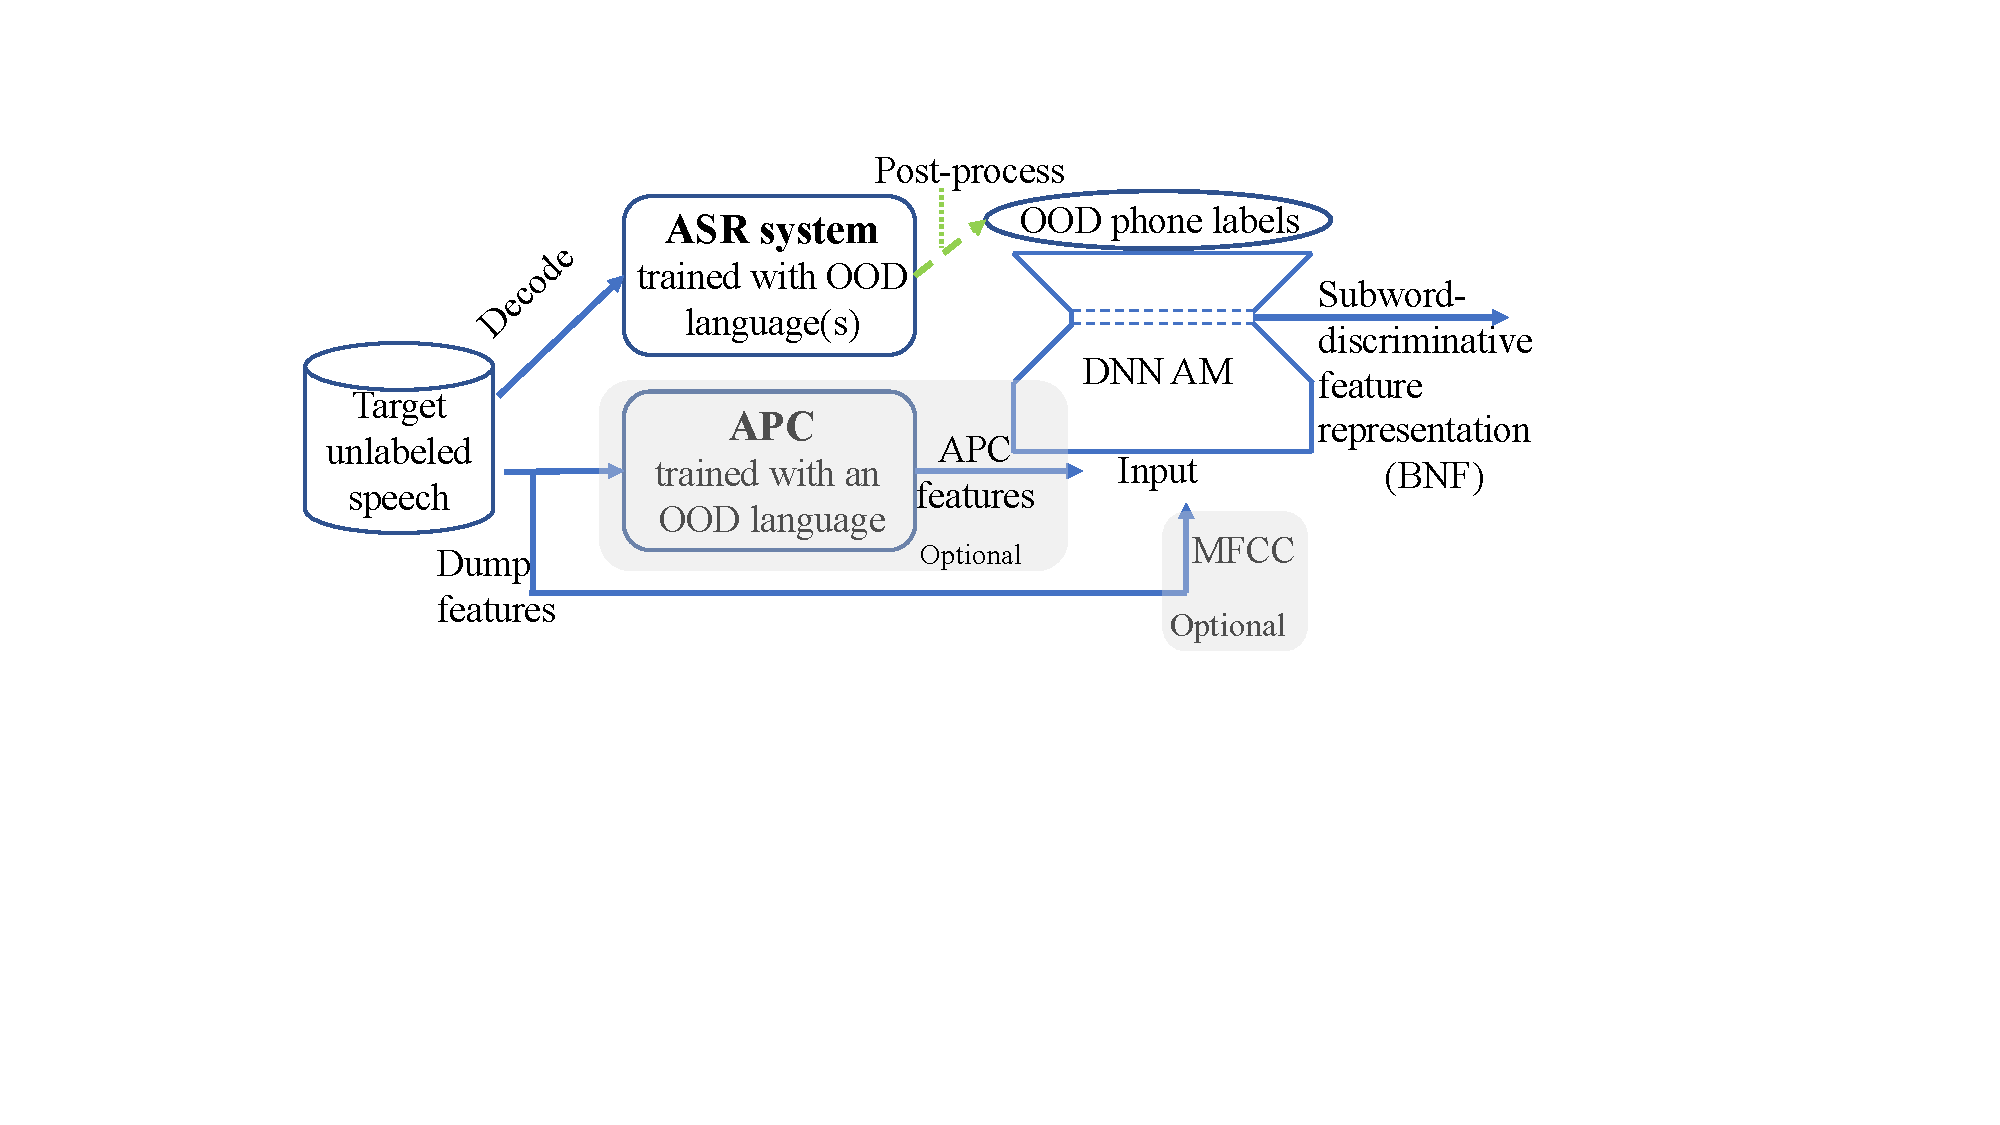
\includegraphics[width =  \linewidth]{LaTeX/USM.pdf}
    \caption{The first stage in the proposed approach. ``OOD'' denotes out-of-domain, i.e. language(s) different from the target language, ``AM'' denotes acoustic model.}
    \label{fig:framework_1st}
\end{figure}
It mainly consists of  an APC model and a  DNN acoustic model (AM). 

APC is a self-supervised learning model without the need of transcriptions for training. It is 
trained to predict a future speech frame $n$-step ahead (named \textit{prediction step}) based on the current and past frames of an utterance \cite{Chung2019}. APC is incorporated in \cite{feng2020unsupervised} to extract \textit{APC features} as input to the DNN AM (see Figure \ref{fig:framework_1st}), owing to its ability to make phonetic and speaker information   in speech   more separable than  MFCC.   \cite{feng2020unsupervised} indicated that the effectiveness of the APC model requires over $50$ hours of target language training data. As this study assumes  an extremely low-resource scenario ($4.5$ hours), it is unknown whether APC is still effective. 
% However the present study assumes  an extremely low-resource scenario with only $4.5$ hours of target (Mboshi) speech.  It remains unknown whether APC is effective with this scenario. 
A recent study \cite{riviere2020unsupervised} found self-supervised models trained on one language   can benefit another language. This  inspires us to compare (1)  using an APC model trained with an OOD language's speech; and (2) bypassing the APC model and feeding MFCC  to the DNN AM (see Figure \ref{fig:framework_1st}). 
% In other words, either the APC features or MFCC features are fed as input to the DNN AM (see Figure \ref{fig:framework_1st}).
% \subsubsection{s}

The  DNN AM in Figure \ref{fig:framework_1st}
% contains a bottleneck layer in the middle.
% Bottleneck features (BNFs)  extracted from a BN layer of a DNN AM are known to carry phonetic information while being largely speaker-independent \cite{vesely2012language_independent}. 
is trained with target language acoustic data, using APC features or MFCCs as input features.
% APC features (or MFCCs) of the target unlabeled speech data. 
Due to the zero-resource scenario, frame-level phone labels required for training the DNN AM are obtained based on an OOD (non-target)  ASR system  \cite{feng2020unsupervised}: Each  target speech utterance is decoded by the OOD ASR system so that every frame is assigned with a  phone label modeled by the OOD ASR. 
By this means, an OOD language's phonetic knowledge is exploited for the target language acoustic modeling.
% the OOD phone labels provide phonetic representation for the target speech from a cross-lingual perspective. 
After training the DNN AM, BNFs are extracted from the bottleneck layer of the DNN as the desired subword-discriminative representation.
% As phoneme inventories  of an OOD language may not completely cover all 

One limitation of the above-mentioned OOD     phone labeling   is that speech sounds in the target language but absent from an OOD language may not be well represented by the OOD phone labels. To  overcome this, we % exploiting multiple OOD languages' resources to 
train a language-independent OOD ASR system leveraging multiple phonetically diverse languages' resources. Notably,  we use International Phone Alphabet (IPA) symbols \cite{international1999handbook}   to represent phones of different OOD languages, making   phone inventories of the multilingual ASR system language-independent \cite{zelasko2020sounds}. This also enables acoustic information sharing of  the same  or  very close\footnote{We understand sounds from two languages with the same IPA symbol may not be entirely the same.}  sounds across different languages, as these sounds are with the same IPA symbols during   ASR  training.   A multilingual ASR system captures a wider phonetic space, thus is expected to provide better OOD phone labels for target speech than a monolingual  ASR system. We compare the use of multilingual versus monolingual OOD ASR systems to generate OOD phone labels for target speech to train DNN AMs and extract BNFs.
% Using the multilingual OOD ASR system to assign IPA phone labels to target speech frames, we will show it provides better phone labels than a monolingual OOD ASR system, which is essential for the AUD task.
% , frames of target speech are assigned with IPA phone labels.  We will show the multilingual OOD ASR system provides better phone labels  for the target speech  than a monolingual OOD ASR system. 

Another modification to the approach in \cite{feng2020unsupervised} is adding a post-processing step to  the OOD ASR based phone labels (see Figure \ref{fig:framework_1st}): we experimentally found that  via training an HMM with the OOD phone labels and Mboshi acoustic data, followed by 
% the OOD phone labels and Mboshi speech are used to train a GMM-HMM, followed by
using the HMM forced-aligned phone labels as supervision to train the DNN AM (instead of directly using OOD phone labels   as DNN supervision \cite{feng2020unsupervised}), the AUD performance is improved. %This post-processing step is .
%Hence this post-processing method is applied throughout this paper.

% , comparing to directly use the OOD phone labels in DNN AM training. 

% As was done in \cite{feng2020unsupervised}, While phone labels generated by an OOD ASR system can be directly taken as supervision to train the DNN AM, 
% We found  improved by first training a GMM-HMM  with Mboshi speech and the OOD phone labels, followed by using the forced-aligned phone labels as supervision for DNN AM training. We adopted the latter method throughout this paper.    
% , and (2) an APC model trained  with an out-of-domain (OOD)  language is effective. In this study we will compare  


% Figure \ref{fig:framework_1st}.
% \todo[inline]{
%   Concise description of IS2020 approach\\
%      emphasize we're using universal IPA phone symbols to train an OOD (multilingual) ASR system.\\
     
%  }

\subsection{Stage 2: speech segment representation and clustering}
\label{subsec:approach_2nd_stage}
This stage builds upon a learned subword-discriminative feature representation by the first stage, and applies $k$-means clustering to   obtain a finite set of clusters, each of which resembles a phoneme-like acoustic unit. The discovered units are the final outcome of the proposed two-stage approach.  

Speech clustering can be realized at segment level \cite{LeeSoongJuang} or at frame level   \cite{chen2015parallel}.  
Segment-level speech clustering   \cite{Bhati2019unsupervised,levin2013fixed} treats each variable-length speech segment as one sample during clustering.
Two main issues in segment-level clustering are the estimation of phone segment boundaries and segment-level feature representation. For the first issue,  we rely on an OOD ASR system (see Section \ref{subsec:approach_1st}):  after decoding  target speech data, phone boundary information is acquired by finding discontinuities of the frame-level OOD phone labels. This phone boundary estimation method is similar to \cite{feng2016exploit}, except we are using a multilingual and  IPA symbol based OOD ASR system.

For the second issue,  several past studies \cite{kamper2017embeded,Bhati2019unsupervised} suggested a \textbf{downsampling}   method \cite{levin2013fixed}: an arbitrary-length speech segment is cut into a fixed number ($s$) of consecutive sub-segments, and 
the averages over frame-level feature vectors within each sub-segment are concatenated 
% within each sub-segment its average over all frame-level feature vectors ($d$-dimension) is calculated,  concatenated 
to form a segment-level feature vector of dimension $s \times d$.
Note that when $s=1$, the method is equivalent to another widely adopted \textbf{average} based method \cite{I3EWang}. The downsampling method with a large $s$ captures abundant temporal information which is not captured by the average method, however a large $s$ leads to a high dimension of the segment-level feature vector which might adversely affect $k$-means. This study compares both methods in obtaining fixed-dimensional segment representation.
%given a speech segment of an arbitrary $t$,  $\{\bm{x_1}, \ldots, \bm{x_t}\}$

% \todo[inline]{Frame-level clustering and pros/cons, state we will compare our segment-level clustering against frame-level one}
% To compare against segment-level clustering, we   
This study implements a frame-level clustering system as a baseline, using the same  $k$-means algorithm and frame-level feature representation. While circumventing the two issues   mentioned above,   frame-level clustering  tends to produce over-fragmented discovered units \cite{wu2018optimizing,feng2019_TASLP}, which we also show in our experiments.  
Moreover, we report an ``upperbound'' segment-level system by assuming the availability of golden phone  boundary information, while keeping the other settings unchanged. This allows us to quantify the performance degradation attributed from imperfect  phone boundary estimation.
%We experimentally validate this and compare against segment-level clustering.

%  \todo[inline]{  leave the investigation of alternative clustering algorithms in this task for future study}
  %Aliquam quis orci consectetur nulla luctus ullamcorper. Suspendisse finibus luctus erat a dapibus.

\section{Experimental setup}
\label{sec:setup}
\subsection{Evaluation metrics}
\label{subsec:setup_eval}
To compare with  past studies, 
% make performance comparable to past studies, 
we use two common metrics in the AUD task \cite{ondel2016variational,Ebbers2017,Yusuf2020hierarchical}: 
% Following recent past studies \cite{ondel2016variational,ondel2017bayesian,Ondel2019Bayesian,Yusuf2020hierarchical}, the AUD performance is evaluated by two metrics from two perspectives. 
normalized mutual information (\textbf{NMI})  \cite{cover1999elements} and \textbf{F-score}. NMI   measures the statistical dependency between discovered units and ground-truth phone units,  (see \cite{Yusuf2020hierarchical} for details). An NMI value ranges between $0$  and $100\%$, with a higher value  indicating a higher consistency between discovered units and phones, hence is preferred. F-score, defined as the harmonic mean of recall (R) and precision (P),  is used to measure  the accuracy of  phone segmentation. A tolerance of $\pm20$ ms is set \cite{Yusuf2020hierarchical} when computing F-score values. Higher F-score, R and P   are preferred. %Both NMI and F-score are calculated based on  

\subsection{Databases}
\label{subsec:setup_database}
The AUD  performance    is evaluated by  Mboshi \cite{Godard2018mboshi}, a corpus
% containing $5,130$ sentences spoken by three speakers, 
with a total amount of $4.5$ hours. Mboshi phone alignments are available, but are not used during   system development. Note that the DNN AM in our system is trained and evaluated on the entire Mboshi data without training-test partition, as we are tackling an unsupervised learning problem. This  is also consistent with   recent  studies in AUD \cite{Yusuf2020hierarchical,Ondel2019Bayesian}.

Speech data used to train OOD multi-/monolingual ASR systems is taken from $13$ languages. In between, $5$ languages are from GlobalPhone  \cite{schultz2002globalphone}: Czech (CZ, $24$ hours), French (FR, $23$ hours), Spanish (SP, $12$ hours), Mandarin (MA, $15$ hours) and Thai (TH, $23$ hours). The other $8$ languages are from IARPA Babel: Cantonese (CA, $127$ hours), Bengali (BE, $55$ hours), Vietnamese (VI, $78$ hours), Lao (LA, $59$ hours), Zulu (ZU, $54$ hours), Amharic (AM, $39$ hours), Javanese (JA, $41$ hours) and Georgian (GE, $45$ hours).

For systems incorporating an APC model in the first stage, data used to train the APC model is taken from the \textit{unlab-600} set ($600$ hours) in  Libri-light (English) \cite{kahn2019librilight}.

% \todo[inline]{Mboshi, 5 GlobalPhone languages and 8 Babel languages. Libri-light unlab-600 (apc when applicable)}
 
% \todo[inline]{NMI, F-score}

\subsection{Implementation of stage 1}
\label{subsec:setup_stage1}
The APC model is trained by  following  implementation details in \cite{feng2020unsupervised}: the model consists of $5$ LSTM layers of dimension $100$ with residual connections between two consecutive layers. The prediction step is $5$. The input features to the APC model is $13$-dimension MFCCs with cepstral mean normalization (CMN). 
% The model is trained for $100$ epochs. 
After training, output from the top layer of the APC model is extracted as the APC features.

The multilingual and monolingual OOD ASR systems used to generate OOD phone labels for target speech data are trained using Kaldi \cite{povey2011kaldi}, adopting a hybrid  architecture \cite{dahl2011context}, following implementation details in \cite{feng2021how}. There are  $2$ multilingual systems and $5$ monolingual systems developed, differing  only in the choice  of   training   languages: \textbf{Multi-5} denotes a multilingual system trained with 5 GlobalPhone languages; \textbf{Multi-13} denotes a multilingual system trained with 13 GlobalPhone+Babel languages; \textbf{Mono-CZ, Mono-FR, Mono-SP, Mono-MA, Mono-TH} are five monolingual systems, each trained with one GlobalPhone language   indicated in their names. All these ASR systems use IPA symbols to represent basic acoustic units, and the mapping from  orthographic transcriptions  to IPA symbol sequences is obtained by LanguageNet G2P models \cite{hasegawa2020grapheme}. The AM adopts a factorized time-delay neural network (TDNNF) consisting of $12$ layers with a hidden dimension of $1024$
% and bottleneck dimension of $128$ 
and Resnet-style skip connections, trained with the LF-MMI criterion \cite{povey2016purely} for $4$ epochs, with a starting learning rate (LR) of $10^{-3}$. The input features consists of $43$-dimension high-resolution MFCC+pitch features and $100$-dimension i-vectors. The language model (LM) is a uni-gram phonotactic LM instead of a much stronger, RNNLM, as we hope the OOD ASR phone labeling process is minimally affected by the OOD language phonotactics. The LM is trained with training data transcripts by SRILM \cite{Stolcke02srilm--}.

% phone labels for target speech generated by an OOD ASR system   mainly reflect acoustic properties rather than OOD language phonotactics. 

% are used to convert orthographic transcriptions in GlobalPhone and Babel corpora into IPA symbol sequences in order to train the ASR  systems. 
The DNN AM is trained by Kaldi with Mboshi acoustic data, using either APC features or MFCC features as input features. 
For each of  the $7$ multi-/monolingual OOD ASR systems, its generated and post-processed (see Section \ref{subsec:approach_1st}) OOD phone labels are used    to train one DNN AM with MFCC as input features, resulting in $7$ DNN AMs. We additionally implement one DNN AM using APC features as input features and \textbf{Multi-13} based OOD phone labels, in order to test the effectiveness of APC in the AUD task.
The DNN AM adopts a similar TDNNF structure to that in an OOD ASR system, except: a $40$-dimension bottleneck layer is  placed below the top TDNNF layer; i-vector input is not included as we found  it worsening the performance; the model is trained for $20$ epochs with a smaller LR of $2.5\cdot 10^{-4}$ to stabilize the training procedure due to only $4.5$ hours of training material\footnote{Speed perturbation based data augmentation techniques was tried but no improvement was found, thus is not applied.}.  After training a  DNN AM, the BNF for Mboshi data is extracted from the bottleneck layer  as the  learned frame-level subword-discriminative representation, and is used as input to the 
% to carry out clustering in the 
second stage of the proposed system.
% \begin{itemize} 
%     \item Multi-5: multilingual OOD ASR system trained with 5 GlobalPhone languages.
%     \item Multi-13: multilingual OOD ASR system trained with 5 GlobalPhone plus 8 Babel languages.
%     \item Mono-CZ, Mono-FR, Mono-SP, Mono-MA, Mono-TH: five monolingual OOD ASR systems, each trained with a GlobalPhone language as indicated in their names.
% \end{itemize}

% \begin{table}[!t]
% % \renewcommand\arraystretch{0.7}
% \centering
% \caption{S.}
% % \resizebox{ 0.9 \linewidth}{!}{%
% \begin{tabular}{l|c|c|cccc}      
% % \hline      
% \toprule
% d\\
% \bottomrule
% \end{tabular}%
% % \footnotetext{`speakers-R/-L' denotes speakers with rich/limited speech data}
% % }
% \label{tab:setup_ood_asr_setting}
% \end{table}


% \todo[inline]{OOD ASR system, DNN AM}

\subsection{Implementation of stage 2}
\label{subsec:setup_stage2}

The $k$-means algorithm is implemented using \cite{scikit-learn}. 
Unless specified, the number of clusters is empirically set as $50$.
% For each segment-level or frame-level clustering, we repeat clustering $5$ times using different  random initialization and report the means and standard deviation of NMI and F-score. 
Segment-level clustering is done towards all the learned subword-discriminative representations by different DNN AMs as mentioned in Section \ref{subsec:setup_stage1}. 
For segment-level clustering, speech segment boundaries are estimated using the OOD ASR system same as the one which is used to generate OOD phone labels in the first stage. 
The downsampling method with $s$ ranging in $\{2,3,4,5\}$ and the average based method are compared in getting fixed-dimension segment  representation. 

A frame-level clustering baseline and an upperbound segment-level system are also implemented, both based on the subword-discriminative feature representation  learned using the \textbf{Multi-13} ASR system in the first stage. Moreover, the effect of setting  the number of clusters ranging between $30$ and $70$ is investigated.
% bet of  segment-level clustering 


% is   implemented, based on the subword-discriminative feature representation  learned using the \textbf{Multi-13} ASR system in the first stage. An ``upperbound'' system 

% is reported by leveraging the golden phone segmentation boundary information, also . %While the upperbound  is \textit{not} an unsupervised AUD system, it  measures the performance gap attributed from imperfect phone segmentation boundary estimation. 
%the best AUD performance our subword-discriminative representation could achieve

 
% \todo[inline]{segment vs frame, num of clusters, upperbound system which makes use of golden phone segment boundary information}

\section{Results and discussion}
\label{sec:results}
For each experiment, we repeat $k$-means clustering $5$ times with different  random initialization and report the AUD performance in means and standard deviation.

\subsection{Multilingual v.s. monolingual OOD ASR systems}
\label{subsec:multi_mono_asr}
\begin{table}[!t]
\renewcommand\arraystretch{0.7}
\centering
\caption{Comparison of adopting multi-/monolingual OOD ASR systems in stage 1 of the proposed approach and SotA. ``\cmark/\xmark'' denotes a system   using APC/MFCC features as input features.  }
\resizebox{ 0.8 \linewidth}{!}{%
\begin{tabular}{c|l|c|c}      
% \hline      
\toprule
APC &   system & NMI ($\%$) & F-score ($\%$)\\
\midrule
\multirow{7}{*}{\xmark}
& Mono-CZ&$40.87\pm0.14$ &$63.01\pm0.06$\\
& Mono-FR&$38.32\pm0.17$ &$\bm{64.14\pm 0.10}$\\
& Mono-SP&$37.57\pm0.51$ &$58.87\pm0.08$\\
& Mono-MA&$38.85\pm0.24$ &$61.45\pm0.12$\\
& Mono-TH&$37.61\pm0.08$ &$61.79\pm0.05$\\
% \midrule
& Multi-5 &$41.93\pm0.28$ &$62.84\pm0.03$\\
& Multi-13 &$\bm{43.00\pm 0.12}$ &$62.89\pm0.07$\\
\midrule
\cmark& Multi-13 &$42.15\pm0.28$ &$62.90\pm 0.15$ \\
\midrule
\midrule
\multirow{2}{*}{N/A}
&Yusuf et al.
\cite{Yusuf2020hierarchical}& $41.07\pm 1.09$ & $59.15\pm 1.51$ \\
&Ondel et al. \cite{Ondel2019Bayesian}& $38.38\pm0.97$ & $59.50\pm 0.78$ \\
\bottomrule
\end{tabular}%
% \footnotetext{`speakers-R/-L' denotes speakers with rich/limited speech data}
}
\label{tab:results_mono_multi}
\end{table}

We first focus on the effectiveness of stage 1 by comparing multilingual and monolingual OOD ASR systems, as well as measuring the effect of using APC features as input features to the DNN AM. In this section,  a fixed setting of  stage 2 is used: segment-level $k$-means; the average based method is used to obtain segment-level feature representation. The performances of our systems and two past works \cite{Yusuf2020hierarchical,Ondel2019Bayesian} achieving state of the art (SotA) are listed in Table \ref{tab:results_mono_multi}. Several observations are made from this table:

(1) Using NMI as the metric, our approach by adopting a multilingual OOD ASR system (Multi-13/Multi-5) significantly outperforms that by adopting a monolingual one. It confirms the efficacy of 
% applying multiple languages' resources to  
building a language-independent OOD ASR system  to provide OOD phone labels for target language DNN AM training, in order to learn a better frame-level subword-discriminative feature representation, comparing to adopting a language-dependent OOD ASR. Using F-score, the system adopting a French   ASR system achieves the best performance, followed by the system adopting  a Czech ASR system. The systems adopting Multi-5 and Multi-13 perform   better than the average over all the $5$ monolingual systems' F-score values ($61.85$).   Since, F-score measures the accuracy of phone boundary estimation, while NMI measures the consistency between the discovered acoustic units and true phone units, the results indicate that the advantage of applying a multilingual OOD ASR system is much more prominent on improving the phonetic relevance of the discovered acoustic units, rather than on improving phone boundary estimation.  

(2) Our best system (Multi-13, MFCC input) performs better than state of the arts \cite{Yusuf2020hierarchical,Ondel2019Bayesian} on both the NMI and the F-score metrics. Similar to our approach,    \cite{Yusuf2020hierarchical,Ondel2019Bayesian} relied on OOD languages' transcribed data during system development. The total amount of OOD data used in  \cite{Yusuf2020hierarchical,Ondel2019Bayesian} was around\footnote{The exact amount was not reported in \cite{Yusuf2020hierarchical}.} $35$ hours (from $7$ languages). While our two best systems (in NMI) exploited more OOD speech data - Multi-13: $595$ hours; Multi-5: $97$ hours, our system Mono-CZ performs on par with or better than \cite{Yusuf2020hierarchical,Ondel2019Bayesian} in NMI and F-score respectively, using only $24$ hours of Czech data.
% are fixed to be   segment-level $k$-means clustering, using the average based method to obtain segment-level feature representation.

(3) The APC model does not benefit the AUD performance (see two Multi-13 systems in Table \ref{tab:results_mono_multi}). By replacing MFCC   with APC features as input to the DNN AM in stage 1, the F-score performance does not differ, while the NMI performance degrades. This observation is partially explained as the lack of sufficient target language (Mboshi) acoustic material: APC is trained with $600$-hour English speech and it fails to transfer knowledge  from English to Mboshi. On the other hand, note that the success of incorporating an APC model in \cite{feng2020unsupervised} was evaluated on a different, USM task, it might be the different task formulation  that leads to ineffectiveness   of APC in this study.

% \todo[inline]{; APC is not effective; multi-13 $>$ multi-5 $>$ mono; probably brief discussion on the use of OOD languages; }

\subsection{Comparison of speech clustering strategies }
\label{subsec:clustering_strategies}
\begin{table}[!t]
\renewcommand\arraystretch{0.7}
\centering
\caption{Comparison of speech clustering strategies in stage 2 of the proposed approach. ``Seg./Fra.'' denotes segment- and frame-level clustering.
``$\ddagger$'' indicates the upperbound system using golden phone boundary information.  }
\resizebox{ 0.99 \linewidth}{!}{%
\begin{tabular}{l|l|c|c|c|c}      
% \hline      
\toprule
Type &System & NMI ($\%$) & F-score ($\%$) & \textoverline{Recall} ($\%$)& \textoverline{Precision} ($\%$) \\
\midrule
\multirow{6}{*}{Seg.}
&AVG &$\bm{43.00\pm 0.12}$ &$62.89\pm0.07$ & $73.47$ & $54.97$ \\
% \midrule
&DS-2 &$\bm{43.00\pm 0.12}$ &$62.87\pm0.07$& $74.22$ & $54.54$\\
&DS-3 & $42.73\pm0.28$ & $62.70\pm0.15$ &$74.12$& $54.32$\\
&DS-4 & $42.49\pm0.27$& $62.47\pm0.10$ &$73.74$&$54.19$\\
&DS-5 & $42.44\pm0.16$& $62.60\pm0.07$ &$74.07$&$54.20$\\
&AVG$^\ddagger$ &{\color{blue}$59.29\pm1.17$}& {\color{blue}$97.73\pm0.06$} &{\color{blue}$95.57$}  & {\color{blue}$100.00$}\\
\midrule
Fra. & F & $41.82\pm0.20$& $43.59\pm0.35$ & $90.38$  & $28.72$  \\
\bottomrule
\end{tabular}%
% \footnotetext{`speakers-R/-L' denotes speakers with rich/limited speech data}
}
\label{tab:results_segment_strategies}
\end{table}
This section focuses on investigating speech clustering strategies in stage 2, i.e. the downsampling method with different $s$ versus the average based method to obtain segment-level representation, comparison of segment- and frame-level clustering, and measuring the performance gap between systems with and without knowing golden phone boundary information. 
A fixed setting of stage 1 is used: Multi-13 OOD ASR system is used to generate OOD phone labels; APC is not adopted. 
Experimental results are listed in Table \ref{tab:results_segment_strategies}. In this table, ``AVG'' denotes the average based method, ``DS-2$\sim$5'' denotes the downsampling method with $s=2\sim5$.
In addition to NMI and F-score, Table \ref{tab:results_segment_strategies} also reports  average  \textit{recall} and \textit{precision} values over $5$ $k$-means repetitions per system, in order to gain deeper insights on the differences between segment- and frame-level $k$-means.

It is clearly seen that all systems adopting segment-level $k$-means achieve better NMI and F-score performances than the frame-level system (F). The superiority of segment-level systems is more prominent on F-score ($19\%$ absolute improvement)  than on NMI ($1.2\%$ absolute improvement). More detailedly, frame-level clustering results in a very low \textit{precision} value, indicating a large proportion of false boundaries  is hypothesized. 
% From the high \textit{recall} and the low \textit{precision},  
This implies a frame-level system tends to over-segment target speech, same to findings in \cite{wu2018optimizing,feng2019_TASLP}.  
% , which adversely affects the discovering of phoneme-like acoustic units, i.e. a worse NMI. 

Table \ref{tab:results_segment_strategies} indicates the downsampling method does not show advantage over a simpler, average based method, and a larger $s$ leads to slight NMI degradation. While relevant studies suggested the downsampling method \cite{kamper2017embeded,Bhati2019unsupervised}, we show that for  such a low-resource Mboshi evaluation database, using $k$-means algorithm,  the average based method is comparable, if not better than, the downsampling method.

Table \ref{tab:results_segment_strategies} shows the upperbound system (AVG$^\ddagger$) outperforms our best system (AVG) by $16.3\%$ absolute NMI increase. The \textit{recall} rate less than $100\%$ is understood as after clustering, some   consecutive segments are assigned with the same index. The   NMI gap is attributed exclusively from the imperfect phone boundary estimation by the OOD ASR system. It is expected that via improved phone boundary estimation, or by adopting an approach to iteratively refining segmentation and target language acoustic modeling \cite{kamper2017embeded}, the  frame-level subword-discriminative representation learned in the first stage  could be used to achieve an NMI performance that approaches the upperbound. 
% A possible reason is the 

% although it does better in \textit{recall} rate ($90\%$) than segment-level clustering. This finding is consistent to 





% \todo[inline]{, mention there were works iteratively modeling unsup units and refining boundaries, which might be used to improve our system.}

\subsection{Effect of the number of clusters}
\label{subsec:number_of_clusters}
\begin{table}[!t]
\renewcommand\arraystretch{0.7}
\centering
\caption{NMI (row 2) and F-score (row 3) performances w.r.t different numbers of clusters (row 1).}
% \caption{Comparison of different numbers of clusters. The three rows denote cluster number, NMI and F-score.  }
\resizebox{ 0.99 \linewidth}{!}{%
\begin{tabular}{ccccc}      
% \hline      
\toprule
$30$ & $40$ & $50$ & $60$ & $70$ \\
% \bottomrule
\midrule
% NMI & 
$41.35\pm0.21$& $42.50\pm0.34$&$43.00\pm0.12$ & $43.22\pm0.52$&$43.20\pm0.53$\\
\midrule
$62.81\pm0.05$&$62.89\pm0.04$ &$62.89\pm0.07$ & $62.77\pm0.14$&$62.76\pm0.10$\\
\bottomrule
\end{tabular}%
% \footnotetext{`speakers-R/-L' denotes speakers with rich/limited speech data}
}
\label{tab:results_num_clusters}
\end{table}
This section measures the effect of setting different numbers of clusters in the AUD task. The same setting of stage 1 used in section \ref{subsec:clustering_strategies} is used here. For stage 2, segment clustering with the average based method is adopted. The numbers of clusters ranging between $30$ and $70$ are tested. Table \ref{tab:results_num_clusters} summarizes the results. It can be seen, 
the optimal number of clusters for NMI ranges between $60$ and $70$. After tuning the number of clusters, an absolute NMI improvement of $0.22\%$ is achieved comparing to setting the default $50$ clusters. 
The F-score performance is less sensitive to the number of clusters than NMI. 
Overall, a number of clusters between $50$ and $70$ is preferred.

% \todo[inline]{  optimal cluster number 50-70. }


% \todo[inline]{Probably a quick overview of discovered acoustic units' statistics? Which true phone(me)s got high results}
\section{Conclusions and future work}
\label{sec:conclu}
This paper addresses the unsupervised AUD task, and proposes a two-stage approach. We show that our approach achieves state of the art on a very low-resource Mboshi database. We confirm the advantage of using a multilingual OOD ASR system over a monolingual one in providing supervision for target language acoustic modeling and in phone boundary estimation, with the former being more prominent. The APC model is found ineffective in the AUD task. Segment-level clustering with   a downsampling method and an average based method both outperforms frame clustering. There is a $16\%$ NMI performance gap attributed from imperfect phone boundary information. The proposed approach achieves the optimal AUD performance by setting a number of clusters around $50$ to $70$.

\section{Acknowledgements}

We thank Lucas Ondel for valuable discussion on the evaluation code resources for the Mboshi database. \\
% Note to authors: Authors should not use logos in the acknowledgement section; rather authors should acknowledge corporations by naming them only.


\bibliographystyle{IEEEtran}
\bibliography{mybib}
 
% \begin{thebibliography}{9}
% \bibitem[1]{Davis80-COP}
%   S.\ B.\ Davis and P.\ Mermelstein,
%   ``Comparison of parametric representation for monosyllabic word recognition in continuously spoken sentences,''
%   \textit{IEEE Transactions on Acoustics, Speech and Signal Processing}, vol.~28, no.~4, pp.~357--366, 1980.
% \bibitem[2]{Rabiner89-ATO}
%   L.\ R.\ Rabiner,
%   ``A tutorial on hidden Markov models and selected applications in speech recognition,''
%   \textit{Proceedings of the IEEE}, vol.~77, no.~2, pp.~257-286, 1989.
% \bibitem[3]{Hastie09-TEO}
%   T.\ Hastie, R.\ Tibshirani, and J.\ Friedman,
%   \textit{The Elements of Statistical Learning -- Data Mining, Inference, and Prediction}.
%   New York: Springer, 2009.
% \bibitem[4]{YourName17-XXX}
%   F.\ Lastname1, F.\ Lastname2, and F.\ Lastname3,
%   ``Title of your INTERSPEECH 2021 publication,''
%   in \textit{Interspeech 2021 -- 20\textsuperscript{th} Annual Conference of the International Speech Communication Association, September 15-19, Graz, Austria, Proceedings, Proceedings}, 2020, pp.~100--104.
% \end{thebibliography}

\end{document}
